%CaseQuad

Air Traffic Control (ATC) offers many opportunities for automation to allow safer and more efficient landing patterns. 
The constraints of ATC are complex and contain many safety rules \cite{}???. 
In this example we formalize a subset of these rules for an autonomous ATC in MTL.
We demonstrate how the smoothed robustness is used to generate control strategies for safely and robustly landing two quadrotors in an enclosed airspace with an obstacle. 
Simulation results with three initial trajectories (for a multi-start) show that the proposed approach outperforms Simulated Annealing and gradient descent on the non-smooth robustness.
\todo[inline]{it's very important that the reader is not confused about the experimental setup. something like "three initial trajecgtories (for multi-start)" is easily confusing. Initial for who? what's multi-start? take a sentence or two to airily and precisely describe the setup and define your terms.}

The specification for the autonomous ATC with two quadrotors is:
{\small
\begin{subequations}
\begin{align}
\Psi &= \eventually_{[0,N]}(p_1 \in \text{Terminal}) \land \eventually_{[0,N]}(p_2 \in \text{Terminal}) \land   \nonumber \\
& \always_{[0,N]} (\neg (p_1 \in \text{Zone}_1) \lor z_1 \in [1,5]) \, \land \nonumber \\
& \always_{[0,N]} (\neg (p_2 \in \text{Zone}_1) \lor z_2 \in [1,5]) \, \land \nonumber \\
& \always_{[0,N]} (\neg (p_1 \in \text{Zone}_2) \lor z_1 \in [0,3]) \, \land \nonumber \\
& \always_{[0,N]} (\neg (p_2 \in \text{Zone}_2) \lor z_2 \in [0,3]) \, \land \nonumber \\
& \always_{[0,N]} (\neg (p_1 \in \text{Unsafe})) \land \always_{[0,N]} (\neg (p_2 \in \text{Unsafe})) \, \land  \nonumber \\
& \always_{[0,N]} (||p_1-p_2||_2^2 \geq d_{min}^2)
\end{align}
\end{subequations}
}
\todo[inline]{$a \implies b$}
\todo[inline]{major source for confusion: $p_i$ are used as positions and in the first half of the paper as atomic propositions. MUST change one or the other. Small $p$'s are used almost universally for atomic propositions, so change the position symbol, in text and in 2 figures.}

Here $p_1$ and $p_2$ refer to the position of the two quadrotors in $(x,y,z)$-space. 
The specification says that, within a horizon of $N$ steps,  both quad-rotors 
\todo[inline]{quad-rotors or quadrotors?}
should: 
a) Eventually land (reach the terminal zone), 
b) Follow altitude rules in two zones, $\text{Zone}_1$ and $\text{Zone}_2$ which have different altitude floors and ceilings $z_i$,
\todo[inline]{tell the reader what's the significance of floor and celing, basically gotta stay in-between}
c) Avoid the $\text{Unsafe}$ set, and d) always maintain a safe distance between each other ($d_{min}$). 

Note that turning the specification into constraints for the control problem is no longer simple. 
This is due to the $\eventually$ operator, which would require a MILP formulation to be accounted for. 
In addition, the minimum separation and altitude rules for the two zones cannot be turned into convex constraints for the optimization. As will be seen below, our approach allows us to keep the non-convexity in the cost function, and have convex (linear) constraints on the optimization problem.

The $\text{Airspace}$ here is a hyper-rectangle in $\mathbb{R}^3$, $[-5,5] \times [-5,5] \times [0,5]$.
The two quadrotors must start in $\text{Zone}_1 = [-5,0] \times [-5,5] \times [0,5]$, which has a ceiling of $5$m m and an enforced floor of $1$m. 
They must eventually reach the terminal set, which is given by $\text{Terminal} = [3,4] \times [3,4] \times [0,1]$.
The terminal set resides in $\text{Zone}_2 = [0,5] \times [-5,5] \times [0,5]$, which has a ceiling of 3m and a floor of 0m.
Finally, the $\text{Unsafe}$ set is a hyper-rectangle $[-1,1] \times [-1,1] \times [0,5]$ in the middle of the air-space
\todo[inline]{be consistent, airspace vs air-space}. 
In simulation, $d_{min}$ is set to $0.2$ m. 
The formula horizon $N$ is set to $20$.
\todo[inline]{I just finished editing this, and now i'm thinking it's not necessary , this whole paragraph...it suffices to say that all the sets, Terminal, Zonei, etc, are hyper-boxes in $\Re^3$. it doesn't matter what they actually are.}

This arrangement of the air-space, where the specifications for altitude ceiling and floors for either zone are in a $A \implies B$ format, is common in ATC (e.g. If holding in progress, go to holding zone and follow holding zone rules) and also allows us to combine the $\text{Airspace}$ with velocity-limits ($[-5,5]^3$) into the set $X$, which is a convex (Polyhedron) set constraint on the state of both quad-rotors, as will be explained below.
\todo[inline]{unnecessary paragraph}

The quad-rotor dynamics are obtained via linearization around hover, and discretization at $5$-Hz. Similar models have been used for control of real quad-rotors with success (\cite{RTSS15}). For simulation, we set the mass of either quad-rotor to be $0.5$ kg. Acceleration due to gravity is $9.8\,ms^{-1}$.
\todo[inline]{seriously? gravity? drop the mass and $g$, it's irrelevant to this exxperiment.} 
The corresponding linearized and discretized quad-rotor dynamics are given as:

{\tiny
\begin{equation}
\label{eq:quad_dyn}
\begin{bmatrix} \dot{x}_{k+1} \\ \dot{y}_{k+1} \\ \dot{z}_{k+1} \\ x_{k+1} \\ y_{k+1} \\ z_{k+1} \end{bmatrix}= \begin{bmatrix} 1&0&0&0&0&0 \\0&1&0&0&0&0 \\0&0&1&0&0&0 \\0.2&0&0&1&0&0 \\0&0.2&0&0&1&0 \\0&0&0.2&0&0&1\end{bmatrix} \begin{bmatrix} \dot{x}_{k} \\ \dot{y}_{k} \\ \dot{z}_{k} \\ x_{k} \\ y_{k} \\ z_{k} \end{bmatrix} + \begin{bmatrix} 1.96&0&0 \\ 0&-1.96&0 \\0&0&0.4 \\0.196&0&0 \\0&-0.196&0\\0&0&0.04 \end{bmatrix} \begin{bmatrix} \theta_k \\ \phi_k \\ \text{T}_k \end{bmatrix}
\end{equation}
}

Here, the state consists of the velocities and positions in the $x,y,z$ co-ordinates. The inputs to the system are the desired roll angle $\theta$, pitch angle $\phi$ and thrust $\text{T}$. 
In a real quad-rotor, a high-frequency low-level controller (not simulated) is responsible for generating rotor speeds to match the desired roll, pitch and thrust (with yaw generally set to be stabilized at $0$). 
\todo[inline]{last sentence not necessary for this experiment. it's almost a full page and no results yet. that's a long lead-up for this experiment...}

The control problem is to maximize the smooth robustness of the specification $\srob_{\Psi}$, subject to the dynamics of two identical quad-rotors, and input limits of $0.5236$ radians (or $30$ degrees) on both roll and pitch, and $\text{T}\in[-1.5,1.5]$, giving us the set $U$. The set $X$ for state limits on either quadrotor is, as defined earlier, the Cartesian product of velocity limits $[-5,5]^3$ and the $\text{Airspace}$ set, i.e. $[-5,5]^3$. Also with respect to the general control problem, \eqref{eq:general_ctrl}, we set $\gamma=0$ and $\delta=0$. This keeps the smooth robustness only in the cost (to be maximized) and allows a fair comparison of the optimization of robustness with other methods. In general, our formulation has linear constraints (dynamics and $X$, $U$) for both quad-rotors, allowing us to easily apply off the shelf optimization solvers.
\todo[inline]{repetitive. get to it. remove this paragraph and replace it with the control problem mathematically, as done for toy example.}
 %, Simulated Annealing and gradient descent, via SQP, on the robustness function.

For simulation purposes, 
\todo[inline]{what other purposes are there?}
we obtain 3 initial trajectories (via solving different linear programs) from the given initial state to the terminal (landing) set. These three trajectories, each of which has negative robustness (i.e. does not satisfy the given specification), serve as three different initial solutions to A) Our approach B) Gradient-descent via SQP, using the actual robustness function as the cost, C) Simulated Annealing with the actual robustness function as the cost. This multi-start approach can be used in practice when there is a fast initial trajectory generator available.
\todo[inline]{re-word in a much more direct style, as follows:}
We used three methods 
\begin{itemize}
	\item SR-SQP, which uses SQP to optimize the smooth approximation to robustness, $\srobf$
	\item R-SQP, which uses SQP to optimize the \textit{true} robustness, $\robf$
	\item SA, which uses Simulated Annealing to optimize the true robustness
\end{itemize}
For each approach, we ran three optimizations, starting from three different trajectories to initialize the optimization. These \textit{initial trajectories} can be obtained in practice by a fast trajectory generator. 
The three initial trajectories all have negative robustness, i.e. they violate the spec.
\todo[inline]{end of blurb. in fact, these three methods should be defined in the previous example, and from that point owards you just refer to them, no need to re-explain them.}
\begin{figure}[t]
\centering
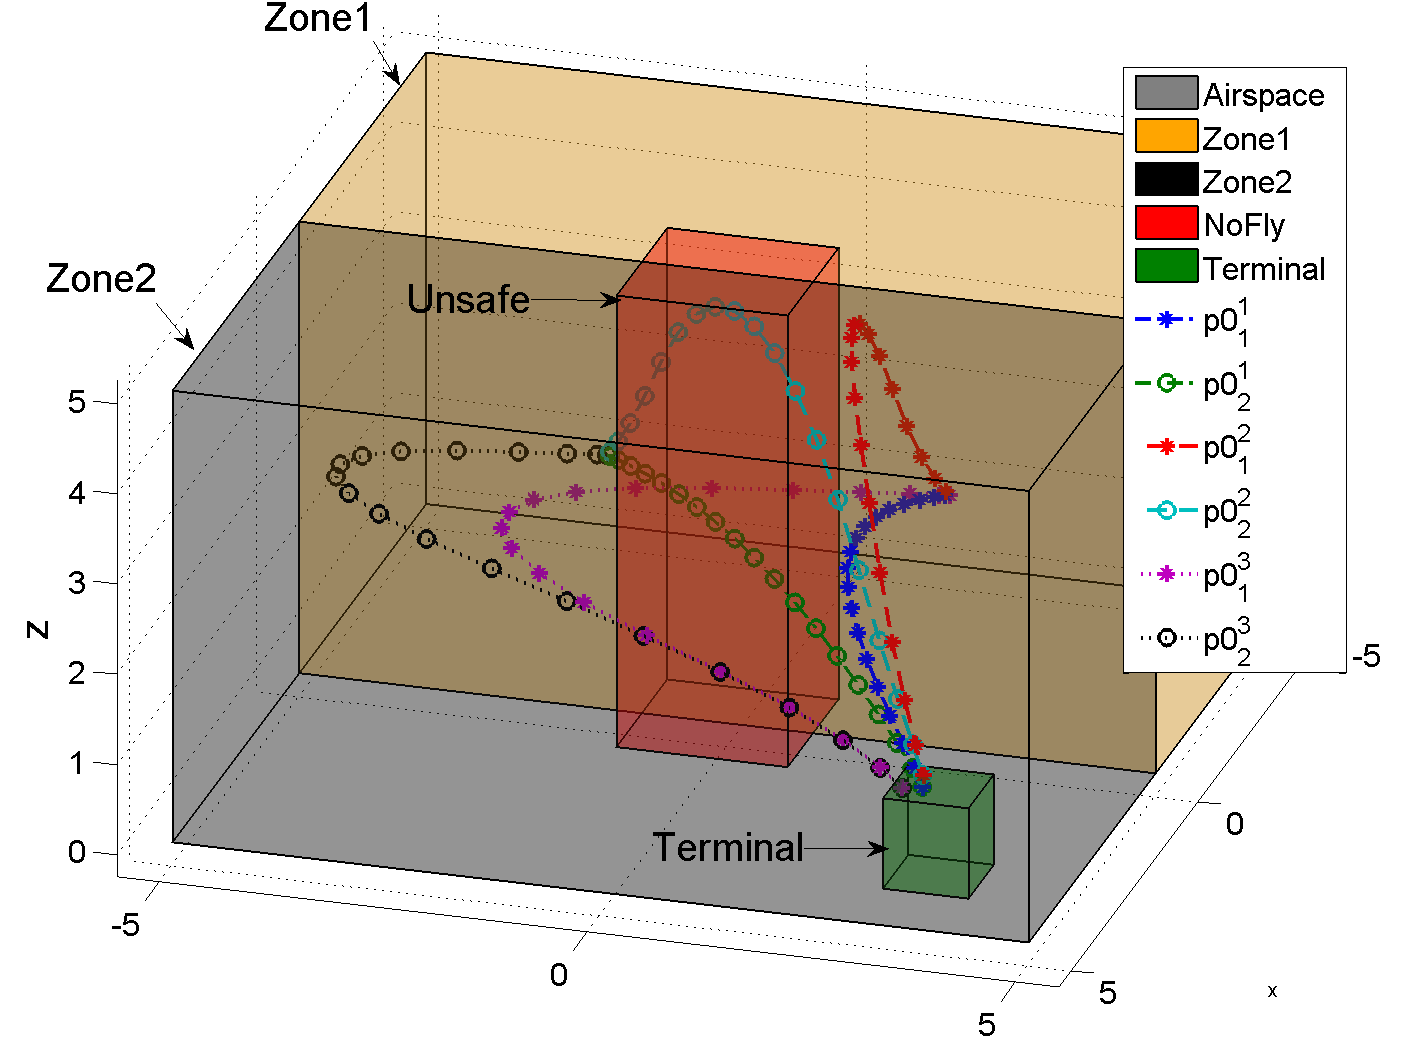
\includegraphics[width=0.49\textwidth]{figures/QuadInitTrajs_scissored}
\caption{The airspace with the corresponding sets, and initial trajectories for the two quad-rotors. Note, all 3 initial trajectories violate the specification. Here, $p0_{i}^j$ refers to the positions of the $i^{th}$ initial trajectory for the $j^{th}$ quadrotor. \todo[inline]{don't foret to change the $p$ into whatever symbol you use. remove sets from teh legend (for next fifgure also)}}
\label{fig:quad_init}
\end{figure}

Fig.\ref{fig:quad_init} shows the initial trajectories for both the quadrotors in the given air-space, neither of which satisfy the specification $\Psi$. 
Fig.\ref{fig:quad_ssqp} shows the three trajectories obtained after applying our control method
\todo[inline]{use the names of the methods, here, SR-SQP} with the three initial trajectories as starting points 
\todo[inline]{it's either a trajectory or a point. the reader can't peer into your head and see that you're thinking about them in the ssame way. Stick to one nomenclature, "initial trajectory". moreover, we've already explained above what an initial rajectory is, so we don't have to keep explaining that it initializes the optim.}
for the optimization, respectively. 
All three trajectories obtained by SR-SQP satisfy the specification $\Psi$. 
To avoid visual clutter, we do not show the trajectories obtained from the other two methods on the figure.
Rather, we summarize them in Table \ref{tbl:opt_performance}. 
Table \ref{tbl:opt_performance} shows the true robustness of the three initial trajectories, and
the true robustness for the trajectories obtained via the three methods. 
Our method, SQP with Smooth Robustness (SR-SQP)
\todo[inline]{define once, use forever: SR-SQP}, 
results in trajectories with the highest robustness.
SA, with an upper limit of 30,000 function evaluations, results in only one trajectory that satisfies $\Psi$. 
SQP on robustness 
\todo[inline]{chicken on rice. R-SQP}
results in trajectories that satisfy $\Psi$ from all 3 initial trajectories. 
R-SQP consistently returns lower values of robustness than SR-SQP, but also from three very initial trajectories, 
\todo[inline]{"very" initial?}
\todo[inline]{re-organize: SR-SQP and R-SQP satisfies the spec every time, SA only once.
	\\ SR-SQP gives highest robustness values, higher than R-SQP.
	\\ observations below about getting stuck at local minima due to non-diff. }
results in trajectories with the same robustness value $0.1798$. 
We conjecture that R-SQP is getting stuck at local minima at points of non-differentiability of the objective, as illustrated in Example \ref{ex:first}.
On further investigation, we also noticed that the robustness value achieved is due to the segment of the $\Psi$ corresponding to $\eventually_{[0,N]}(p_2 \in \text{Terminal})$, i.e. gradient descent does not drive the trajectory deeper inside the set $\text{Terminal}$, unlike our approach, even though the minimum separation property is far from being violated. This lends credence to our hypothesis of SQP terminating on a local minima (which is indeed the flag MATLAB's optimization gives).
\todo[inline]{this last discussion is important. break down your sentences, clarify it, take it easy. you've done the work, don't rush the explanation.}


\begin{figure}[t]
\centering
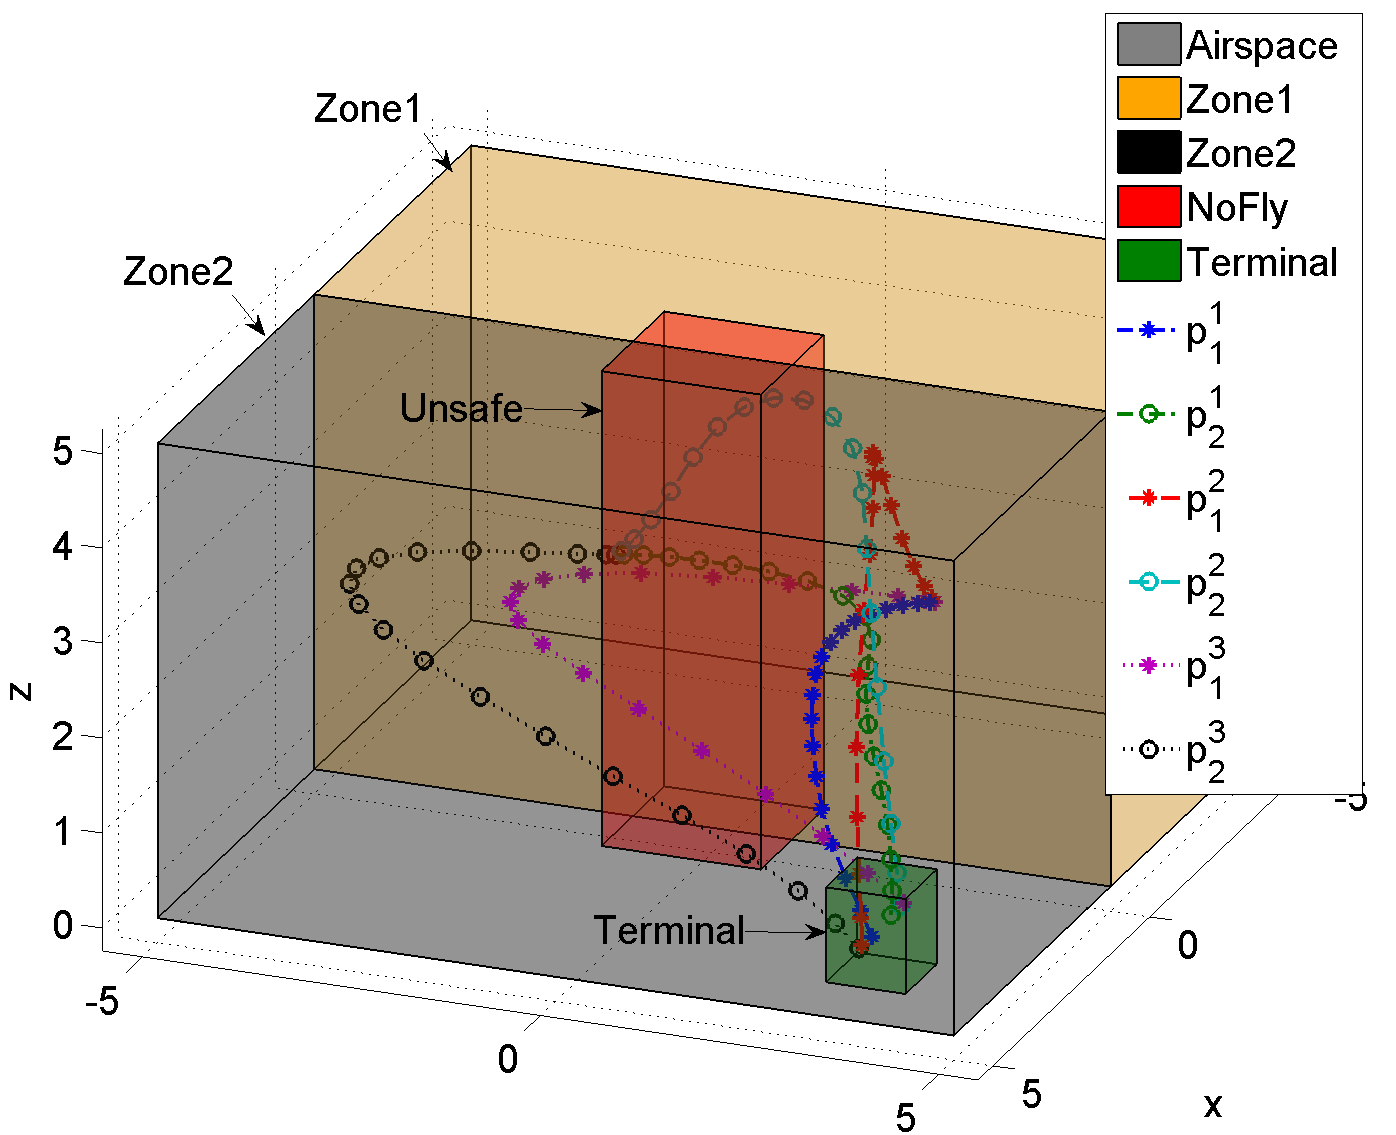
\includegraphics[width=0.49\textwidth]{figures/QuadTrajs_scissored}
\caption{ Trajectories obtained via SQP on smooth robustness, with three different initial trajectories acting as initial solutions for the SQP. Note, all 3 trajectories satisfy $\Psi$. Here, $p_{i}^j$ refers to the positions of the $i^{th}$ initial trajectory for the $j^{th}$ quadrotor.}
\label{fig:quad_ssqp}
\end{figure}

{\small
\begin{table}[htb]
\begin{center}
\caption{Optimization performance}
\label{tbl:opt_performance}
\begin{tabular} {|c|c|c|c|c|}
	\hline
	\textbf{Traj.} & $\rob(\sstraj_0) $ & SR-SQP: $\rob(\sstraj) (\srob)$ & SA: $\rob(\sstraj)$ & SQP: $\rob(\sstraj)$\\ \hline
	1 & -0.8803 & \textbf{0.2985} (0.2460) & -0.2424 & 0.1798 \\ \hline
	2 & -0.7832 & \textbf{0.3255} (0.3103) & -0.5861 & 0.1798 \\ \hline
	3 & -0.0399 & \textbf{0.2967} (0.2652) & 0.0854 & 0.1798 \\ \hline
\end{tabular}	
\end{center}
\end{table}
}


%\todo[inline]{%Start by motivating the example as something more than a dumb system. E.g. "Air traffic control offers many opportunities for automation to allow a more efficient and safer landing patterns. The constraints of air traffic control are complex and contain many safety rules. In this example we express these rules in MTL and demonstrate how the smoothed robustness is used to generate control strategies for safely and robustly landing two quadrotors. The proposed approach outperforms Simulated Annealing and gradient descent on %the non-smooth robustness."	Then you give the details below}
%1. We take a quad-rotor model with linearized dynamics around hover, similar to those used in \cite{}. The case study involves centralized control of two quad-rotors, with operational objectives given as an MTL specification, and a constrained air-space.

%1.b. Give model, constraints, specification. Shrinking horizon (fixing history) approach applicable (cite Vasu paper)

%2. With the given specification, standard control approaches involving polyhedral constraints are hard to apply because of the temporal aspect of the eventually operator involved. While the two (if-then) altitude rules in the specification can be coded as polyhedral constraints on the set, it would result in a non-convex constraint set for positions. Similarly, the minimum distance between two quad-rotors can also be moved to the constraints but would result in another non-convex constraint if we choose to do so. In our formulation, the non-convexity remains in the cost-function while the constraints are linear.

%3. For simulation purposes, we use obtain 3 initial trajectories (via solving different linear programs) from the given initial state to the terminal (landing) set. These three trajectories, each of which has negative robustness (i.e. does not satisfy the given specification), serve as three different initial solutions to A) Our approach B) SQP using the actual robustness function as the cost, C) Simulated Annealing with the actual robustness function as the cost. This multi-start approach can be used in practice when there is a fast initial trajectory generator available.

%3.b. parameters for simulation annealing and citation for it.

%4. Fig shows the initial trajectories for both the quadrotors in the given air-space. Fig. shows the three trajectories obtained after applying our control method, with the three initial trajectories as starting points for the optimization, respectively. 

%5. Table shows for the three trajectories, initial robustness, robustness for trajectory obtained via the three methods (and the approximate robustness when applicable). In addition, we also tested out simulated annealing with the smooth robustness function in the cost (with the first initial trajectory), resulting in a trajectory with a final cost of blah (approximate robustness of blah).
